\textbf{PROBLEMA 2}
\vspace{20px}

\newcommand{\ivec}{\boldsymbol{\hat{\imath}}}
\newcommand{\jvec}{\boldsymbol{\hat{\jmath}}}
\newcommand{\kvec}{\boldsymbol{\hat{k}}}

Tres alambres infinitos paralelos entre sı́ y perpendiculares al plano de la hoja se ubican en los vértices de
un cuadrado de lado $d$. Uno de ellos lleva corriente $2I$ que entra al plano, mientras que los otros llevan corriente
$I$ que emerge del plano de la hoja.\\

\begin{enumerate}[label=\alph*.]
    \item Calcule el vector campo magnético en el punto $P_1$.
    \item Calcule la fuerza que actúa sobre una carga $q$ con velocidad $\mathbf{v} = 3 \ivec
    + 2 \jvec  + \kvec$̃ situada en $P_1$.
    \item Supongamos que se traslada una carga desde el punto $P_1$ al punto $P_2$ a lo largo de la lı́nea recta que une
    esos dos puntos, ¿cuál es el trabajo que cuesta dicho traslado?
\end{enumerate}

\begin{center}
    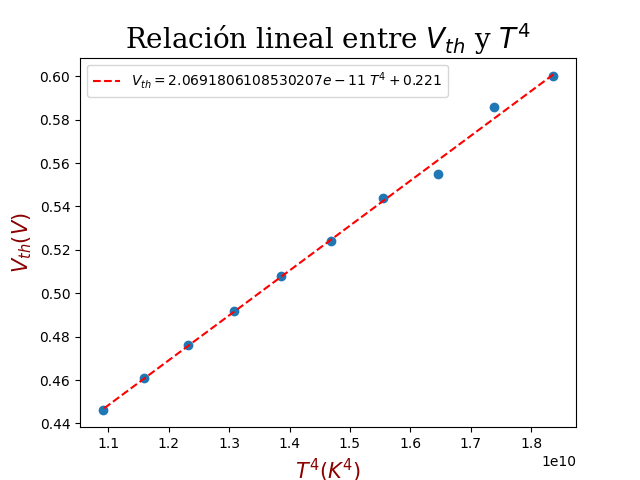
\includegraphics[width=10cm]{files/img2}
\end{center}

\vspace{20px}
\textit{Solución:}
\\